\title{Лекция 13\\Представление в базе знаний онтологий}
\author[]{Шункевич Д.В.}
\institute[]{Белорусский государственный университет информатики и радиоэлектроники}

\begin{frame}
	\titlepage
\end{frame}

\begin{frame}{\\Содержание лекции}
	\topline
	\justifying
	Понятие онтологии. Классификация онтологий. Интегрированная онтология. Связь онтологий и предметных областей. Связь понятия онтологии и семантической окрестности. Представление в базе знаний.
\end{frame}

\begin{frame}{\\Понятие онтологии}
	\topline
	\justifying 
	\begin{SCn}
		\scnheader{онтология}
		\scnidtf{формализация концептуализации предметной области}
			\begin{scnindent}
				\scnrelfrom{ пояснение}{концепт означает понятие}
			\end{scnindent}
		\scnidtf{система понятий, описывающих свойства предметой области}
		\scnheader{sc-онтология*}
		\scnidtf{спецификация (формальное описание) предметной области}
		\scnrelto{второй домен}{онтология}
			\begin{scnindent}
				\scnrelfrom{первый домен}{предметная область}
			\end{scnindent}
		\scniselement{вид знаний}
	\end{SCn}
\end{frame}

\begin{frame}{\\Классификация онтологий}
	\topline
	\justifying 
	\vspace{10mm}
	\begin{SCn}
		\scnheader{sc-онтология}
		\scnsuperset{структурная спецификация}
		\begin{scnindent}
			\begin{scnrelfromset}{пример}
				\scnitem{максимальный класс объектов исследования\scnrolesign}
				\scnitem{класс объектов исследования\scnrolesign}
				\scnitem{частная предметная область*}
				\scnitem{родственная предметная область*}
			\end{scnrelfromset}
		\end{scnindent}
	\scnsuperset{теоретико-множественная спецификация}
	\begin{scnindent}
		\begin{scnrelfromset}{пример}
			\scnitem{включение*}
			\scnitem{разбиение*}
			\scnitem{свойства отношений}
			\scnitem{пересечение*}
		\end{scnrelfromset}
	\end{scnindent}
	
	\end{SCn}
\end{frame}

\begin{frame}{\\***}
	\topline
	\justifying 
	\vspace{10mm}
	\begin{SCn}
		\scnheader{sc-онтология}
		\scnsuperset{терминологическая спецификация}
		\begin{scnindent}
			\begin{scnrelfromset}{пример}
				\scnitem{идентификаторы}
				\scnitem{правила идентификации}
			\end{scnrelfromset}
		\end{scnindent}
		\scnsuperset{логическая спецификация}
		\begin{scnindent}
			\begin{scnrelfromset}{пример}
				\scnitem{логические высказывания и формулы}
				\scnitem{теоремы и аксиомы}
				\scnitem{логическая иерархия понятий}
					\begin{scnindent}				
						\scnitem{понятия, на основе которых строится данное понятие}
						\scnitem{понятия, которые определяются на основе данного}	
					\end{scnindent}
			\end{scnrelfromset}
		\end{scnindent}
		
	\end{SCn}
\end{frame}

\begin{frame}{\\Онтология}
	\topline
	\justifying 
	\vspace{5mm}
		\begin{SCn}
		\scnheader{sc-онтология}
		\scnidtf{объединение семантических окрестностей определенного вида, описывающих свойства всех понятий, исследуемых в заданной предметной области}
		\begin{figure}[H]
			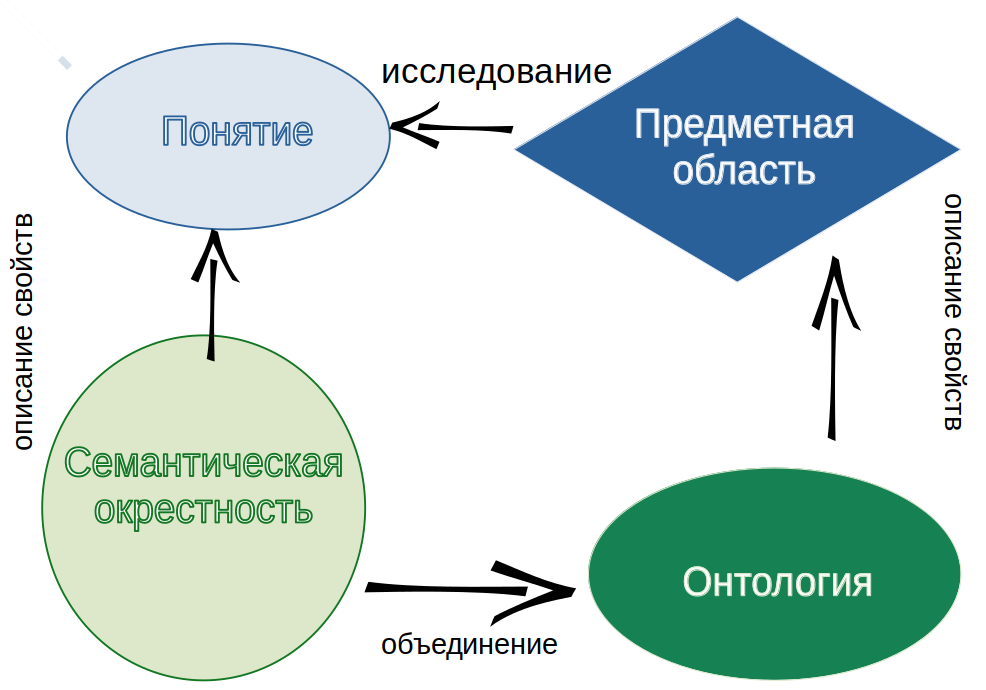
\includegraphics[scale=0.2]{./figures/sd_ontologies/ontology.png}
		\end{figure}
	\end{SCn}
\end{frame}

\begin{frame}{\\Интегрированная онтология}
	\topline
	\justifying 
	\begin{SCn}
		\scnheader{интегрированная онтология}
		\scnidtf{объединение всех видов онтологий}
		
	\end{SCn}
\end{frame}

\begin{frame}{\\}
	\topline
	\justifying 
	\vspace{10mm}
	\begin{figure}[H]
	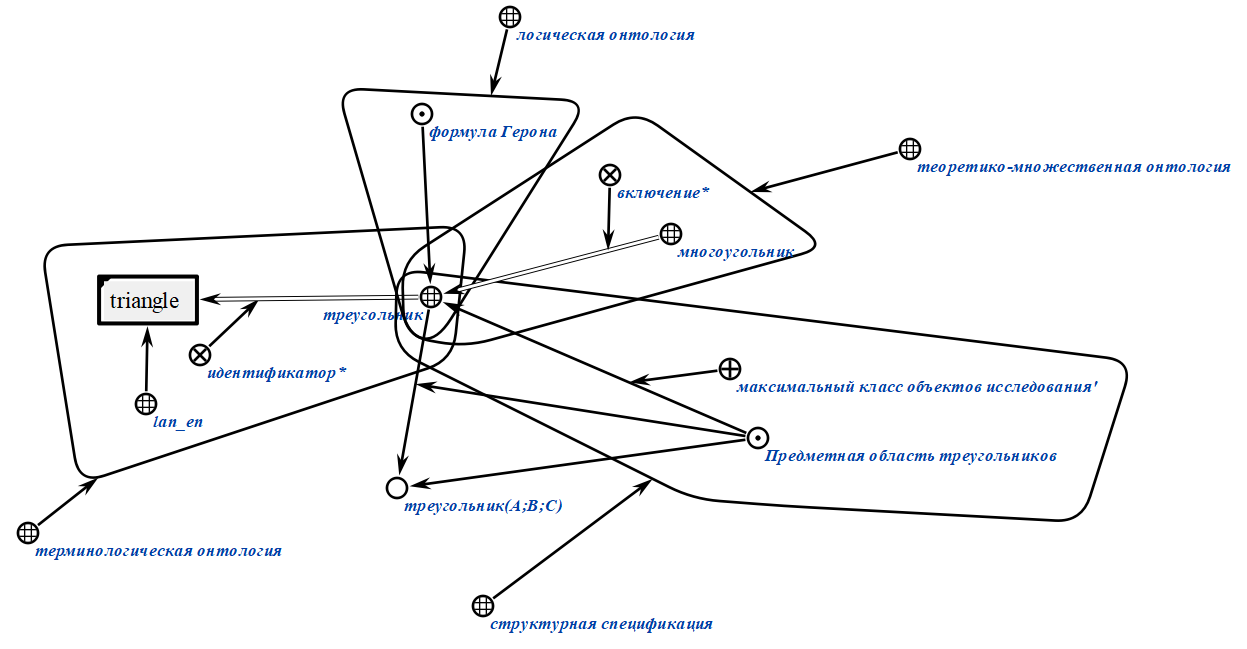
\includegraphics[scale=0.3]{./figures/sd_ontologies/ontology1.png}
	\caption{Пример}
	\end{figure}
\end{frame}

\begin{frame}{\\}
	\topline
	\justifying 
	\vspace{10mm}
	\begin{figure}[H]
		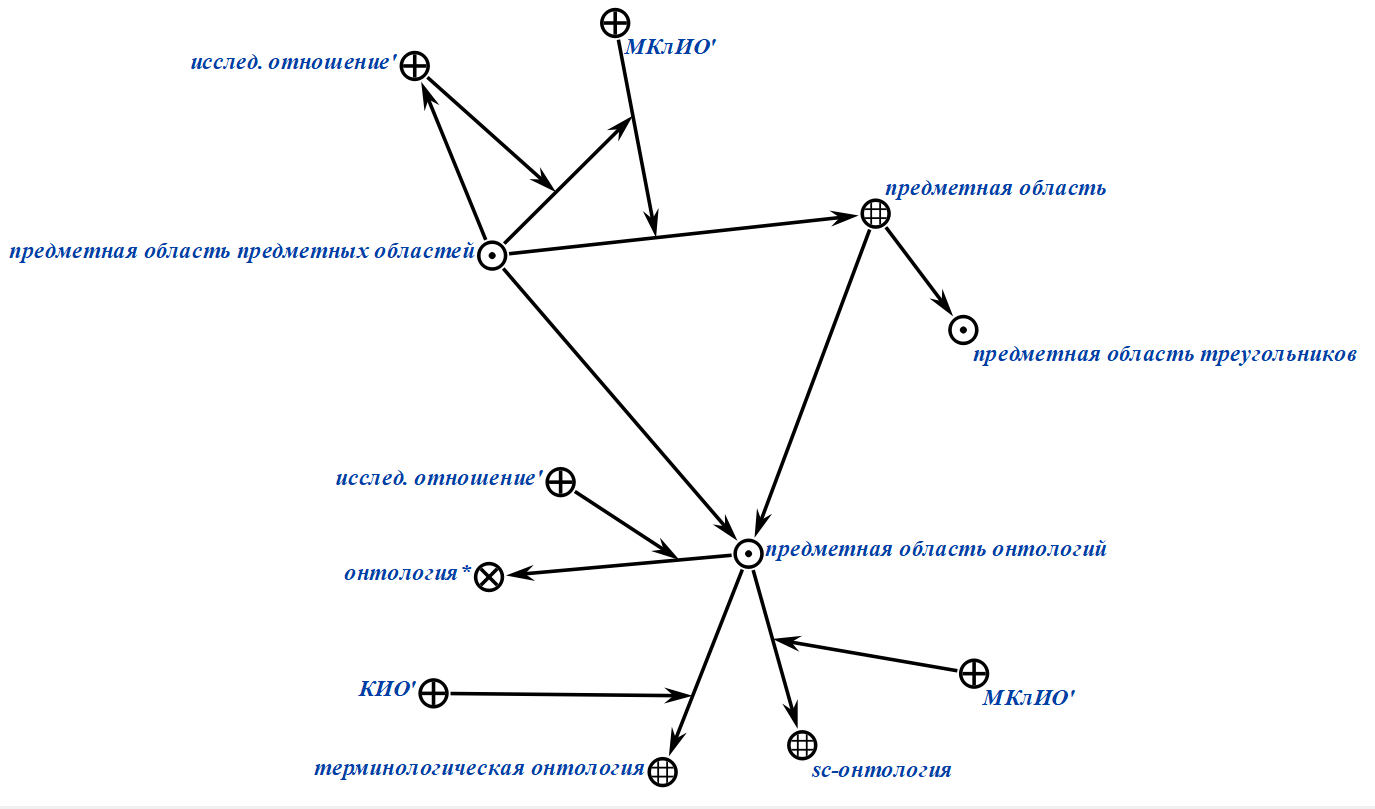
\includegraphics[scale=0.2]{./figures/sd_ontologies/ontology2.png}
		\caption{Пример}
	\end{figure}
\end{frame}

\begin{frame}{\\}
	\topline
	\justifying 
	\begin{figure}[H]
		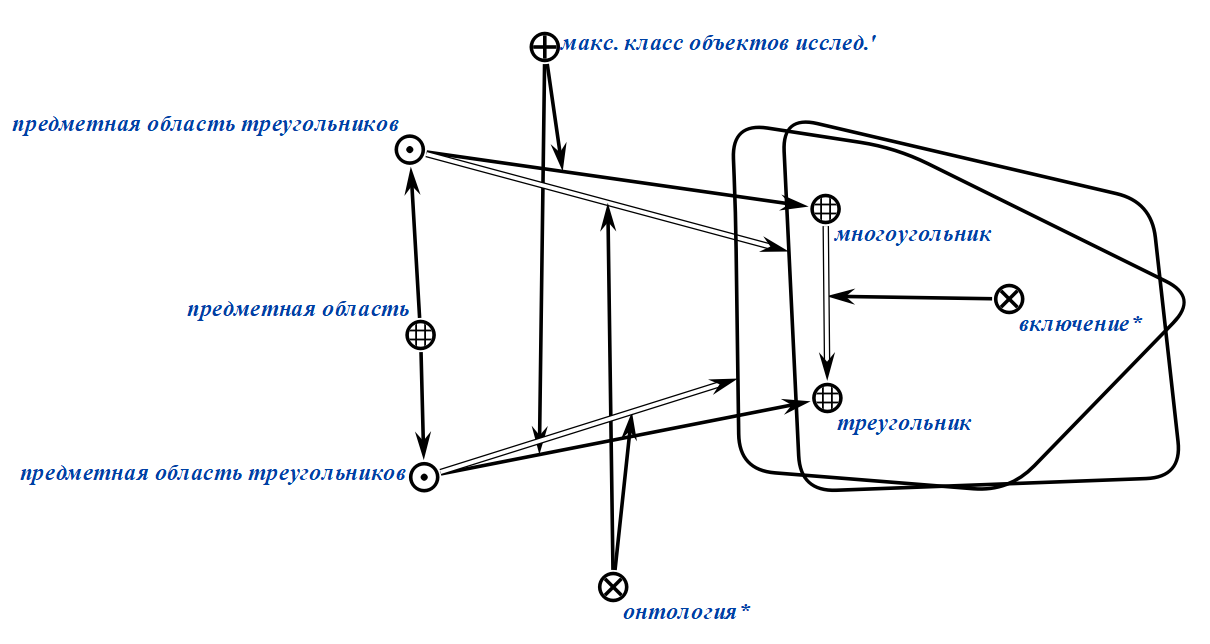
\includegraphics[scale=0.3]{./figures/sd_ontologies/ontology3.png}
		\caption{Пример}
	\end{figure}
\end{frame}
